\documentclass{acm_proc_article-sp}

\usepackage{amsmath}
\usepackage{verbatim}
\usepackage{textcomp}
\usepackage{graphicx}
\usepackage{subcaption}
\usepackage{url}
\usepackage{multicol}
\usepackage{tikz}
\usetikzlibrary{positioning}
\usepackage{wasysym}
\usepackage{mathtools}
\DeclarePairedDelimiter{\abs}{\lvert}{\rvert}
\setlength{\parindent}{1cm}
\usepackage{indentfirst}


\begin{document}

\title{Montreal Real Estate Pricing \\
{\normalsize Code available at: \url{https://github.com/mike-n-7/ML4}}} 
\subtitle{}

\numberofauthors{2} 
\author{
% 1st. author
\alignauthor 
Michael Noseworthy \\
	\affaddr{260512169}
% 2nd. author
\alignauthor Benjamin La Schiazza\\
	\affaddr{260531181}
}

\date{Dec3}

\maketitle
\begin{abstract} %

	One of the most important stages most people go through at one point in their lives involves buying or selling a home.  Real estate is the largest asset the average person will ever own and many times functions as not only a shelter but also an investment. The more information parties on either side of the transaction can obtain, the better their decision will be and the risk of losing large sums of money will decrease. While many models have been applied to this market over the years, not many have investigated the role municipal infrastructure has on pricing these homes. Through the use of data available through the city of Montreal and a snapshot of the real estate market on the island through select agencies, we look to investigate the impact leveraging municipal data can have on pricing and compare the performance of Linear Regression, Lasso Regression and K nearest neighbours within this setting. The best result obtained with one of the algorithms was a mean absolute error of \$44,000. Results show that much of the city data played little in the output of the learners used and that poorer performance by the algorithms suggests the truly non-linearity of the problem space.
	
\end{abstract}

\section{Introduction} %

	The real estate market is one of the most important markets in the modern economy because of the nature of the goods exchanged. Shelter is a fundamental human need and therefore there is a collective interest in pricing homes correctly. While there are other factors in play, an ill-informed party on either side of the transaction can be burned for non-trivial sums. Any insight into pricing homes properly and consistently would be of great interest to all parties involved. 
	
	A house is often the largest investment a person will make in their lifetime. The amount of money used to buy this house is non-trivial and thus great care must be taken in not only choosing the right house, but making sure it's priced appropriately. Estimating housing prices however is not for the faint of heart! To accurately estimate the price of a house, one not only requires an understanding of the housing market (a dynamic and volatile entity), but a deep understanding of the property itself. This knowledge is usual held solely by real estate agents. If we can capture this domain knowledge by using openly accessible data, then this knowledge suddenly becomes accessible to the average citizen who can thus make informed decisions without relying on an expert who unfortunately may not always be acting in their best interest.
	
	On the side of the real estate agents, being able to accurately price a home through automated means of a machine learning algorithm with easily available data will offer new insight into what people are looking for in a house. They can thus spend more time focusing on creating successful pitches to sell the houses as well as make recommendations to clients.
	
	The city of Montreal should also be interested in studies such as this. If we can find a set of city infrastructure that is correlated with the price of a house, it is worth time investigating this correlation. Although correlation does not imply causality, the results can be examined to determine what kind of infrastructure citizens want to find close to home and direct future development efforts towards these areas.
	
	There have been a number of attempts to model real estate prices using Machine Learning approaches. One of the efforts that was of interest involved pricing Boston suburban homes \cite{bostonres}. The results from this study were very impressive and influenced our choice of features for our data. They explored the use of a Linear SVM regression and a partial least squares regression. The former yielded a means-squared error (MSE) of \$10,000 while the latter had a MSE of \$25,000. The interesting point however from their paper is their feature set which included distance to radial highways, density of non-retail businesses in the area as well as local crime rate. These results assured us that decent results have been achieved with the above model in a comparable city and serves as a benchmark for the results that follow. 
	
	The goal of this project was to attempt to model Montreal homes in its various boroughs while using open-data from the city of Montreal \cite{data}. Not wanting to simply repeat results that have been obtained before, and ultimately constrained by the data sets at our disposal, we opted to explore the use of different characteristics in describing and modelling homes in the city. We hope to investigate the role of other municipal infrastructure in determining the value of homes and in doing so, convince policy makers that the collection, aggregation and dissemination of municipal/city data can be beneficial to residents.

\section{Problem Definition and Description of data} %
	
	This project aims to model Montreal housing prices based on a specific set of features in order to determine their importance in marketing a home. As there are all sorts of real estate available on the market, we focused on homes and condominiums. We wanted to explore the role that municipal infrastructure has on the prices of homes, something that hasn't been explored in much depth. It is hence a regression task to determine the price of a property.
	
	Our data samples consist of standard descriptions of each property as well as the number of various municipal establishments within 3 kilometres of the property. This radius was chosen because it represents what we feel is a comfortable walking distance whether it is within the heart of the city or in a suburb. The learning algorithms used include traditional Linear Regression, Lasso Regression and K-nearest neighbours (which seemed appropriate!). 

\subsection{Data} %

	The real estate market, unlike other traditional markets, does not have a centralized trading "floor" or venue. Parties have the option to deal with an agent or sell the house on their own. As a result price information on available properties isn't centralized. All of the housing data had to be retrieved from brokerage web sites. DuProprio (duproprio.com) and Royal Lepage  (royallepage.ca) web sites were used to get the data needed. They did not offer convenient API's so the sites had to be scraped for the necessary data. While this provided all the standard descriptors of properties, datasets released by the city of Montreal were needed to locate police stations, family-friendly buildings, handicap friendly buildings as well as numerous other notable infrastructure. The complete list can be found in the Appendix. Coordinate information for both properties and these entities were used to count instances within a walking radius. For each house, a new feature was added encoding the number of each type of infrastructure within the given radius.
	
	In all 9717 data points were collected. Data points with abnormally high prices (defined in our case as >\$750000) were removed as they were outliers and could adversely affect the results of regression and generalization. As alluded to, the main features were property descriptors (eg. type of property, living area, neighbourhood, latitude, longtitude, number of bathrooms, number of bedrooms etc...) and counts of local municipal infrastructure (eg. fire stations, police stations, monuments, emergency shelters, family quality buildings...). There were 39 features in all and the full list can be found in the appendix.
	
\subsection{Missing Data} %

	Because our dataset was scraped off of websites, there was a lot of data missing. These websites do not hold strict standards as to which features must be included in a house listing and which features may be excluded. Thus not every listing will include all the features we want to include in our model. Figure \ref{fig:missingdata} shows the number of entries that were missing each feature. Note only features with missing data are shown in this figure. Intuitively, these features will have an impact on predicting house price; for example a house with greater living area can be expected to cost more than a similar house that has less living area. 
	
	Another source of missing data we do not consider but would like to mention comes from the Montreal Open Data. We assume that the datasets used are complete and up-to-date when this may not in fact be the case. To derive useful predictions from these features we require accurate knowledge of where infrastructure is located. A potential draw back of this study is that the Montreal data is not historical whereas our house listings are. Therefore the amount of infrastructure in the neighbourhood of a house may be different than how it was back when the house was for sale. This highlights the importance of the city maintaining a time sensitive and up-to-date record of their open data.
	
	The algorithms we chose to apply are not amenable to missing data. Both linear regression and k-nearest neighbours expect to see a value for each feature. Naively replacing this missing data with a value of zero or an inappropriate value can have an adverse effect by creating outliers in the data and generating more noise. We do not wish to remove features that include missing data as this will hurt the richness of our dataset and be detrimental to our predictive ability.
	
	We decided to look at 3 approaches to dealing with missing data: removing instances with missing data altogether, predicting missing data using Expectation Maximum \cite{EM} and predicting missing data with the mean of the features. 
	
	\begin{figure}[h!]
   		\centering
  		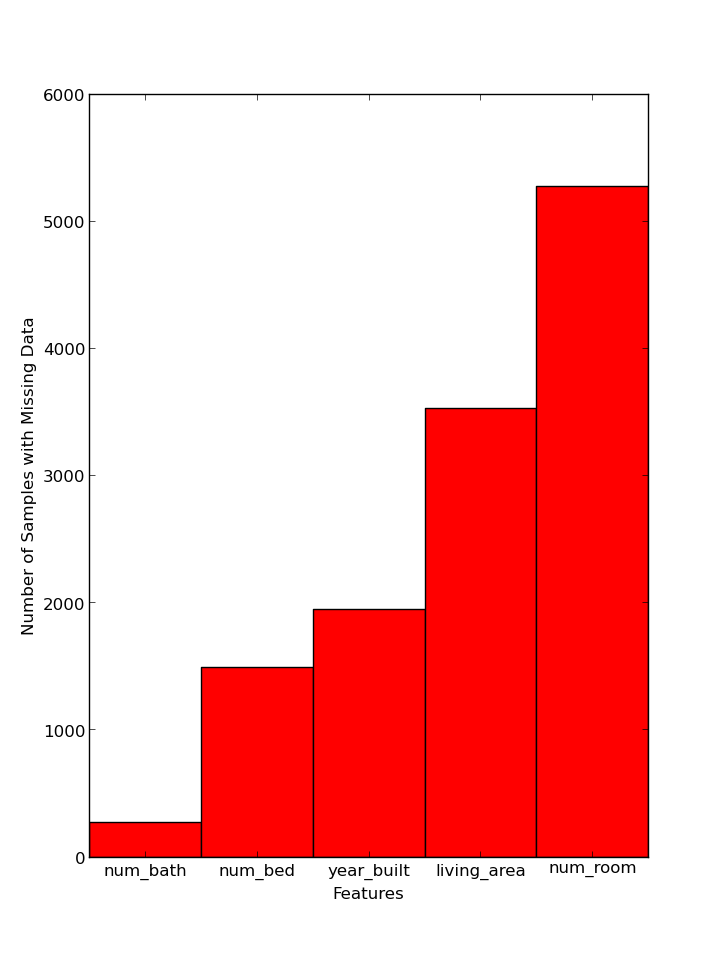
\includegraphics[width=\linewidth]{missing_data.png}
    		\caption{Number of instances with the above features missing. }
    		\label{fig:missingdata}
	\end{figure}
	
	By removing instances that included missing data, we reduced our dataset size to 2289 entries. This dramatic decrease is worrisome as we are losing more than half our data. Thus we also investigate how we can estimate the values of the missing data.

	The simplest method of imputing missing data is by taking the mean of each feature from the instances that are not missing that feature. Then we replace each missing observation with its respective mean. Although this method allows us to keep all of our data, we are effectively adding bias to the data which may be detrimental to our predictive power.
	
	Finally, we try to estimate missing values by using an expectation-maximization like approach. We start by giving each missing value a default value, say its feature's mean. Then we repeatedly try to train a probabilistic model and estimate the values of the missing data until the values converge. In our implementation of this method, we use the scikit-learn MultinomialNB model to estimate missing data. For each feature that has missing data, a model is built using the other features trying to predict the missing feature. Then we use that model to re-estimate the missing data. Note the main limitations from this model arise from the assumptions of the Naive Bayes algorithm. For this method to be effective, the conditional independence assumption must hold and the other features must to rich enough to predict the features with missing data.
	
\section{Methodology} %
	
	Due to the fact that there was a significant amount of missing data, we investigated not only algorithm performance but also methods for treating the missing data. Each algorithm was run with each of the methods for handling missing data. Algorithms were optimized for better results on training sets and a held out test set was used for final evaluation. To select the best method of removing missing data and for tuning hyper-parameters, 5-fold cross validation was used. When the missing data imputation required statistics from the data (EM and mean imputation), the model was generated on only the training data and then these models were used to impute the values of the test data.
	
\subsection{Features} %
	
	Features consisted of two broad categories, property descriptors and integer counts of the number of instances of municipal infrastructure within walking distance from the data point. Many of the features were inherently numerical so they remained untouched. Categorical data such as the property type (house, condo etc...) or the year it was sold (2002-unsold) could have been encoded using integer codes. Research has shown however that one-hot encoding yields better results. \cite{onehot} This is because there is no inherent linear relationship between each category and one parameter cannot capture the relationship between all the categories. These two characteristics hence exploded into a set of binary features.
	
	Feature selection was implicitly done within the Linear Regression and Lasso Regression algorithms. This allowed for non-influential features to be weeded out from the pricing model developed.
	
\subsection{Algorithm Selection} %
	Below is a brief description of the algorithms considered. They were chosen from a wider set of algorithms because during initial smoke testing they had the best results and showed promise. 
	
\subsubsection{Linear Regression} %
	Linear Regression is a simple and classic method that fits a line/plane through the data in the space of features. It's hypothesis for a feature space with m features is of the form, \\
	\[  f_{w}(x) = w_{0}  + \sum_{j=1:m}w_{j}x_{j} \] \\

	The w's are the weights that need to be solved for. Different approaches exist for picking these weights optimally. The scikit-learn implementation uses least-squares which seeks to choose a weight vector to minimize,
	\[ Err(w)  = \sum_{i=1:n}(y_{i} - w^{T}x_{i})^{2}\] \\
	
	A closed form solution does exist but the remaining details, while interesting, are not pertinent, and gradient descent is a numerical method commonly used to tackle this problem. Linear regression is an algorithm of interest to us not only because it is a common method used for economic modelling, but it has an intuitive interpretation. Based on the magnitude of the weights, we can tell which parameters most influence the price of a house and whether there is a positive or negative correlation. The goal of this paper is to do exactly this.
	
\subsubsection{Lasso Regression} %
	Lasso Regression is similar in nature to Linear Regression but makes a number of improvements. It is a form of \emph{regularization} which aims to impose constraints on a solution to prevent overfitting. In Lasso Regression, the weights are constrained by penalizing their absolute value. This forces less important features to have weights of 0 and implicitly weeds out useless features in the process. Because the real estate domain is a bit foreign to us, we simply included features we felt might have influence on property price. This algorithm will help trim them down to a relevant subset.
	
	It solves for a weight vector s.t. \\
	\[ w^{lasso} = argmin_{w}(\sum_{i=1:n}(y_{i} - w_{0} - \sum_{j=1:m}x_{ij}w_{j})^{2} + \lambda\sum_{j=1:m}\abs{w_{j}}) \]
	
	
\subsubsection{K Nearest Neighbours} %
	K nearest neighbours takes a different approach. The core assumption made with this method is that examples with similar feature vectors should have similar outputs. Neighbours of a queried datapoint should be used to determine its value and not points that are far away. In a regression task, once the neighbours have been located, the mean of their values (or a weighted average) is taken to assign to the queried point.
	
	The scikit-learn implementation takes a basic average of the neighbouring data to predict new values. This method is very intuitive but performance really can depend on the nature of the data involved. In our case it seems like a very good option because homes tend to be priced similarly to homes in the same (literal) neighbourhood. Beyond the fact that the algorithm's name seems apt, it should be able to capture this assumption regarding real estate as literal neighbours will have similar construction dates, sizes and proximity to infrastructure.
	
	Being a lazy learner, K nearest neighbours has a strong dependency on the actual dataset. This means the the way we come up with missing data is important as a poorly estimated value can push an otherwise close point farther away. The distance function is also of large importance to this method. By default scikit-learn uses the Minkowski distance,
	\[ d(x, y) = (\sum_{i=1}^n | x_i - y_i|^p)^{\frac{1}{p}} \]
	
	 By default p=2 and thus this reduces to the Euclidean distance. This may not be the best choice for the metric as elaborated upon in the discussion.

\subsection{Implementation Details} %

	Raw data had to be scraped from real estate websites. To do so we used the popular Scrapy framework available for python \cite{scrapy}. A spider was written for each website and data from each was loaded through a script into a cohesive raw dataset. This raw data was then cleansed by removing outliers and bad data and extended using the Montreal datasets as discussed previously. All scripts for collecting and pre-processing of data is available in the code base. Montreal data was downloaded and then parsed for coordinate information. Whenever an address was supplied instead of GPS coordinates, the Google Maps API was used to retrieve the corresponding longitude and latitude.
	
	All the algorithms used were implemented in the scikit-learn library \cite{scikit}. It provides efficient implementations of many useful algorithms and procedures and therefore we wanted to take advantage of the fact that it is available for use. Beyond the implementations of the regression algorithms, it was also used to set up our K sets for our K-fold cross-validation procedure. 

\section{Results} %
	 The results were generally a bit disappointing when compared to the benchmark paper referenced in the Introduction \cite{bostonres}. Analysis however offers many plausible reasons for this as well as interesting insights. 
	 
\subsection{Linear Regression}
	Figure \ref{fig:linreg} compares the performance of Linear Regression over the three datasets representing approaches to handling missing data. Results from cross-validation can be seen in table  \ref{fig:linregres}. Best performance was with the malformed data removed and yielded a mean absolute error of \$44,680 on the held out test set.

	 \begin{figure}[!htbp]
   		\centering
  		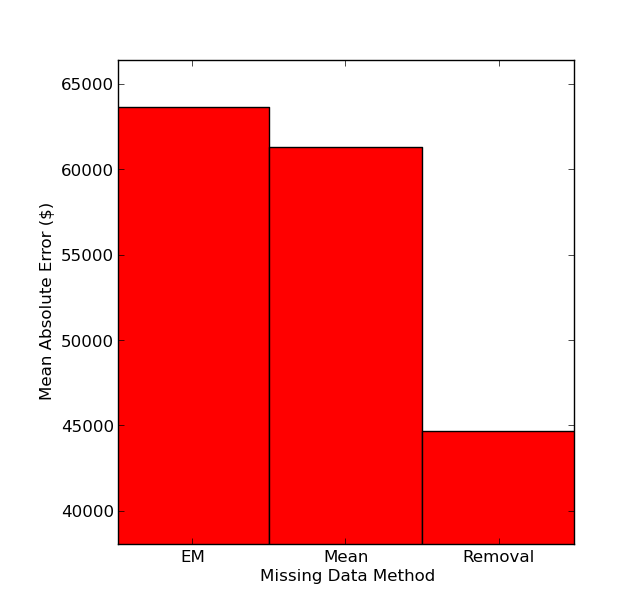
\includegraphics[width=\linewidth]{linear_regression_tuning.png}
    		\caption{Performance of Linear Regression algorithm}
    		\label{fig:linreg}
	\end{figure}
	\begin{center}
	
    \begin{table}	
    \begin{tabular}{| l | l |}
    \hline
    Missing Data Method & Mean Absolute Error \\ \hline
    \hline
    Removal & 44680 \\
    \hline
    Mean Imputation & 61335 \\
    \hline
    Expectation Maximization & 63672 \\
    \hline
    \end{tabular}
    \caption{Mean absolute error for linear regression using various methods to handle missing data.}
    \label{fig:linregres}
    \end{table}
\end{center}
\subsection{Lasso Regression}
	For lasso regression, along with testing each missing data method, we also optimized the regularization hyper-parameter, $\lambda$. However, performance seemed to be only marginally affected. Figure \ref{fig:lassoreg} shows once again that removing the missing data was most fruitful. Best mean absolute error was approximately \$44,315 using a$ \lambda$ value of 100 on the held out test set.
	
	 \begin{figure}[!htbp]
   		\centering
  		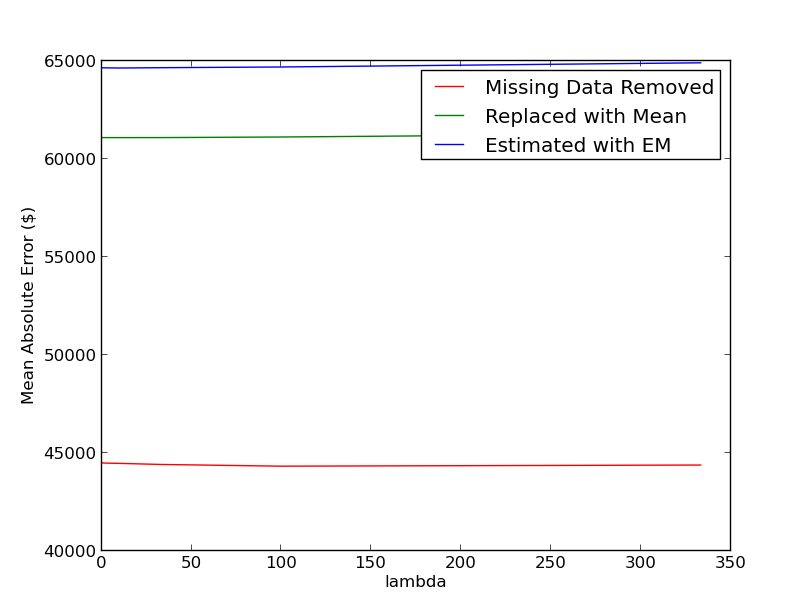
\includegraphics[width=\linewidth]{lasso_tuning_plot.png}
    		\caption{Performance of Lasso Regression algorithm}
    		\label{fig:lassoreg}
	\end{figure}
	
	\begin{center}
	\begin{table}	
    \begin{tabular}{| l | l | l |}
    \hline
    Missing Data Method & $\lambda$ & Mean Absolute Error \\ \hline
    \hline
	Removal & 0.1 & 44485 \\
	\hline
	Removal & 0.3 & 44482 \\
	\hline
	Removal & 1 & 44477 \\
	\hline
	Removal & 3 & 44469 \\
	\hline
	Removal & 10 & 44457 \\
	\hline
	Removal & 33 & 44402 \\
	\hline
	Removal & 100 & 44315 \\
	\hline
	Removal & 333 & 44373 \\
	\hline
    Mean Imputation & 0.1 & 61080\\
    \hline
 Mean Imputation & 0.3 & 61079\\
 \hline
 Mean Imputation & 1 & 61079\\
 \hline
 Mean Imputation & 3 & 61079\\
 \hline
 Mean Imputation & 10 & 61078\\
 \hline
 Mean Imputation & 33 & 61079\\
 \hline
 Mean Imputation & 100 & 61109 \\
 \hline
 Mean Imputation & 333 & 61279 \\
    \hline
    Expectation Maximization & 0.1 & 64640\\
    \hline
Expectation Maximization & 0.3 & 64640\\
\hline
Expectation Maximization & 1 & 64639\\
\hline
Expectation Maximization & 3 & 64636\\
\hline
Expectation Maximization & 10 & 64629\\
\hline
Expectation Maximization & 33 & 64645\\
\hline
Expectation Maximization & 100 & 64682\\
\hline
Expectation Maximization & 333 & 64895 \\
    \hline
    \end{tabular}
    \caption{Mean absolute error for lasso regression using various methods to handle missing data and tuning the regularization parameter.}
    \label{fig:lassores}
    \end{table}
\end{center}
	
\subsection{K Nearest Neighbours}
	The optimal K was 5, as shown in Figure \ref{fig:knn}. Once again simply removing the missing data yielded the best results. Complete summaries of tuning parameters can be found in table \ref{fig:knnres}. On the held-out test set, a mean absolute error of \$45,131 was achieved.
	
	\begin{figure}[!htbp]
   		\centering
  		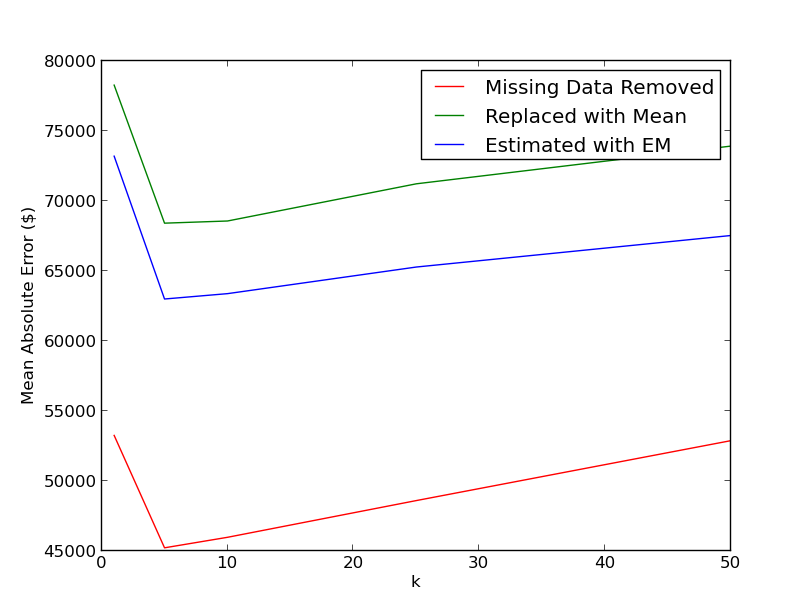
\includegraphics[width=\linewidth]{knn_tuning.png}
    		\caption{Performance of K-Nearest Neighbours as a function of K}
    		\label{fig:knn}
	\end{figure}
	\begin{center}
	\begin{table}	
    \begin{tabular}{| l | l | l |}
    \hline
    Missing Data Method & k & Mean Absolute Error \\ \hline
    \hline
	Removal & 1 & 53237 \\
	\hline
Removal & 5 & 45209\\
\hline
Removal & 10 & 45960\\
\hline
Removal & 25 & 48585\\
\hline
Removal & 50 & 52868\\
	\hline
    Mean Imputation & 1 & 78259\\
    \hline
Mean Imputation & 5& 68398\\
\hline
Mean Imputation & 10 &68553\\
\hline
Mean Imputation & 25 &71210\\
\hline
Mean Imputation & 50& 73907\\
    \hline
    Expectation Maximization & 1 & 73183\\
    \hline
Expectation Maximization & 5 &62981\\
\hline
Expectation Maximization & 10 &63364\\
\hline
Expectation Maximization & 25 &65266\\
\hline
Expectation Maximization & 50 &67519\\
    \hline
    \end{tabular}
    \caption{Mean absolute error for kNN using various methods to handle missing data and tuning the number of neighbours.}
    \label{fig:knnres}
    \end{table}
\end{center}
\subsection{Feature Selection}
	A major driving force of this project was to determine whether the data provided by the city of Montreal was useful in pricing homes across the island. Would the location of certain infrastructure help in the prediction of the worth of a particular property? Two of the algorithms tested above implicitly rank the features by assigning weights to each feature dimension. The higher the magnitude of the weight, the more important it is in determining price. Figure \ref{fig:feats} shows how Linear Regression and Lasso Regression treated each of the 38 features. 
	
	 \begin{figure*}[!htbp]
   		\centering
  		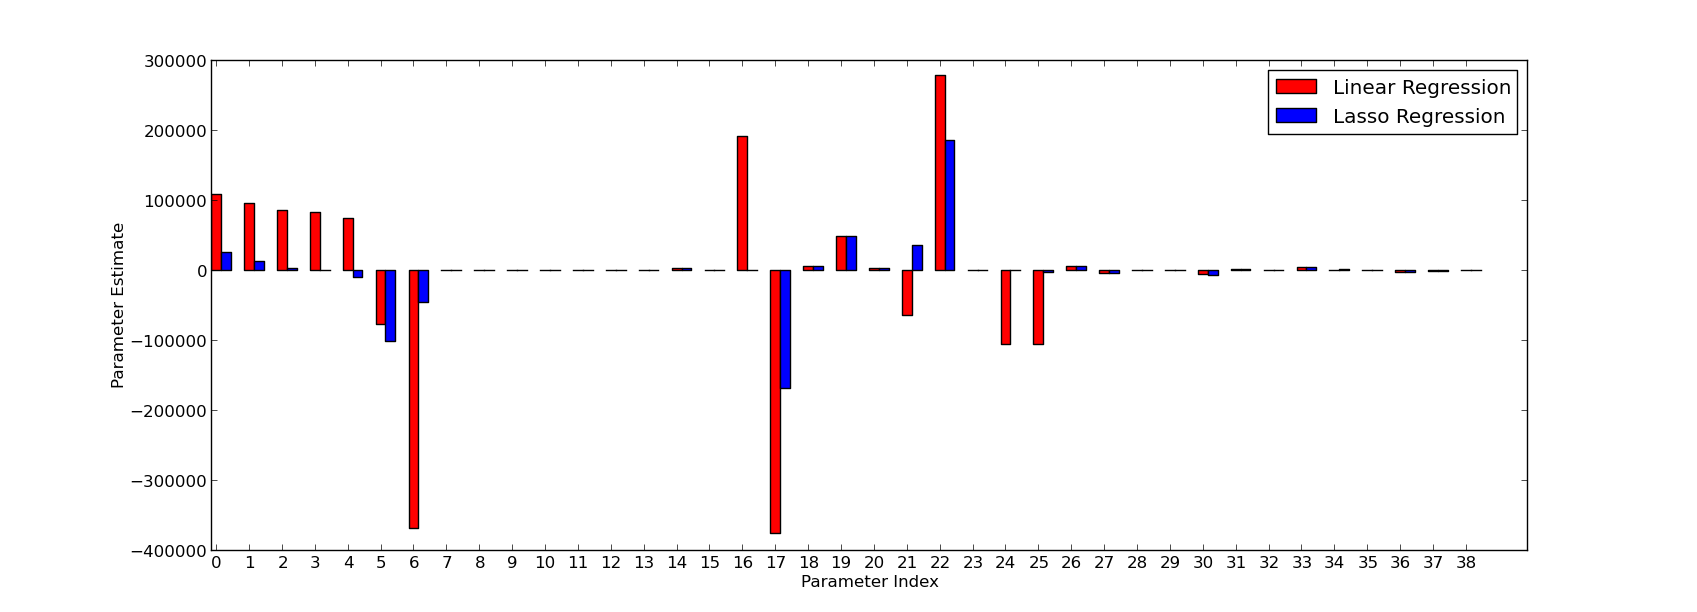
\includegraphics[width=\textwidth]{parameter_values.png}
    		\caption{Parameter/Weight values for each feature for Linear and Lasso Regression.}
    		\label{fig:feats}
	\end{figure*}
	
	The list full list of features is included in the Appendix. Generally speaking however the features in the middle are the core descriptions including living area, year built, latitude and longitude. To the right are the features constructed from the city data. The features to the left are a one hot encoding of the year the property sale was completed.

\section{Discussion}

\subsection{Analysis} %
	The results generally were not as great as was expected. The paper referenced in the introduction \cite{bostonres} gave us hope that we may be able to achieve similar results. The use of a distinctly different feature set however may be the main reason why the mean absolute error obtained in our experimentation was not comparable. However, this comparison should be taken lightly as since the features as well as the data domain (Boston vs. Montreal) are different, the results cannot be directly comparable. A number of insights were gained from all this experimentation. The first is regarding the algorithms chosen. At the start, smoke testing convinced us that all three algorithms were contenders. Ultimately they were all very close in performance, albeit relatively poor for this domain. Linear regression performed marginally better, in the end this is not significant.
	
	Regarding the Linear algorithms (Linear Regression and Lasso Regression), their poorer performance could be attributed to the non-linearity of the problem space. The housing market is incredibly complex as is evident by the fact that no one quite understands it very well. The feature sets curated and experimented with did not seem to encapsulate the necessary information needed to predict the correct prices. The nearest neighbours shortcomings may have been in the density of the data. The majority of the data came from taking a snapshot of the Montreal real estate market on a couple of brokerage sites. Intuitively similar homes that are close to each other (literally) should be priced similarly but the fact that all the houses in a neighbourhood simply don't go up for sale all at once presents problems when leveraging the proximity of data points in the feature space. One weakness of the k nearest neighbours approach is that we used the standard Euclidean distance metric. This is naive and may not be the best metric for the question at hand (ie. which houses are similar). Instead, we could design our own distance metric. One that prioritizes physical distance to get houses in the same neighbourhood, and then looking at the other features to find similar houses in that neighbourhood.
	
	A second aspect of our experimentation was in the way we handled missing data. As the root raw data was scraped off of sites, there were many holes. Of the three methods for handling such cases, surprisingly the best one was to simply remove them from the dataset. This drastically reduced the dataset to about the third of the size. One of the hypotheses we came up with was that properties with complete data generally came from certain types of properties (eg. location). There was less noise and as a result a model could be fit with greater ease. Another reason that removal of missing data may have performed better than the other two methods is that the other two methods make assumptions of the data that may not hold. For mean imputation, we could have introduced too much bias into the dataset to yield good performance. Indeed this method has its criticisms \cite{meancrit}. As for our expectation-maximization like method, the Naive Bayes' assumption of conditional independence may not hold, or the data may not be inherently linearly separable. There is also a possibility that that other features may not be rich enough to provide good estimates for missing data.
	
	The last main goal was to determine whether the data from the city, locations of municipal infrastructure, would influence prices in any way. As can be seen in Figure \ref{fig:feats}, they were not very influential. It is somewhat reassuring to see living area or year of construction get more importance because that is in line with our expectation. The features with the highest magnitude of weights include latitude, longitude, number of bathrooms, house type, as well as which year it was sold. Generally there is understandably a lot of variability in the prices of comparable homes (according to our feature set). Homes are renovated (which adds value), left to ruin, made with specific materials, lie in different zoning areas etc... It would be interesting to see how our experimental results differ if given access to some of these other characteristics. 
	
\subsection{Contribution, Limitations \& Future Work}
	As alluded to above, we hypothesize that given more information about homes and properties in the city of montreal, our approach would be more fruitful. We are confident that analysis of the composition of the local neighbourhood (walking distance) as well as the core descriptors of a home would be sufficient in modelling the real estate market for residential use. The current data provided by the city of Montreal was not influential enough to construct such a model but as has been shown \cite{bostonres}, it is not out of the question that socially sensitive data (crime rates) and others (building material) would play a bigger role than the location of police and fire departments. Thus we encourage the city of Montreal to continue curating and releasing more open data, as it can only benefit experiments like these.
	
	We have been able to show that interpolating observations to fill in missing data is not always appropriate in this setting as there is so much variability in properties, despite the fact that observable characteristics (location) are similar. Future work would definitely involve rigorously collecting more complete data regarding properties around the island as well as collecting and using more municipal data to truly determine what is important for buyers when purchasing a home. With more data, we may be able to build better models for imputing missing data. When designing future experiments, it will also be useful to consider not only what will provide a rich feature set for predicting house price (as we did), but also consider which additional features may offer better predictive power for imputing missing data. One large drawback to point out is the correlation between missing features. For example number of rooms is clearly correlated to the living area in a house, however many samples were missing both these features.
	
	We would also like to point out the relevance of the one-hot encoded historical date (ie. in which year the property was sold). Being a dynamic market, it was expected that time would have a large impact as to how much a house would cost. Thus future research should investigate other methods for modelling the time-dependencies of the housing market such as an autoregressive model.
	
	There is a need to have a more centralized database or resource for real estate in the city (or any city). Building materials, crime rates, locations of public buildings and other crucial information should be collected and made available to the public to inform potential buyers as well as level the real estate market playing field. Such knowledge can be extremely beneficial to the average resident so that they can make informed decisions on either side of a transaction (Note: We haven't consulted any real estate brokers however to confirm if they would benefit from this open data model). Forgetting about machine learning for a minute, we can see that this data by itself is incredibly useful. When buying a house, it is a common practice to do research on the neighbourhood. However, the sparsity of the needed data can make this seemingly trivial task extremely time consuming. Providing this information at a centralized hub would be of great value not only to data analysts, but also to the average citizen.

\section{Conclusion}

	Overall, simple linear regression performed the best when predicting the price of a house. The infrastructure features available from the city of Montreal did not prove useful in predicting the price of a house, however we believe this is due to the nature of the features, and other features that Montreal could release would provide more insight \cite{bostonres}. We encourage the city to continually curate and maintain datasets with a high standard in order to improve models such as these. 
	
	The features that proved most interesting when predicting the price of a house include the house's location, number of bathrooms, the type of house, as well as when the house was sold. Including historical information modelled by time dummy variables allowed us a much greater insight into the housing market.
	
\section{Appendix}
We hereby state that all the work presented in this report is that of the authors.
\subsection{Feature Index Mapping}
Used to interpret Figure \ref{fig:feats} \\

\begin{tabular}{ l | r }
  0 & Not Sold \\
  1-13 & Year Sold \\
  14 & Number of beds \\
  15 & Year Built\\
  16 & Longitude\\
  17 & Latitude\\
  18 & Number of rooms\\
  19 & Number of bathrooms\\
  20 & Living Area (mxm)\\
  21-25 & Property Type (house, plex, chalet, loft, condo)\\
  26 & Number Parking Spots\\
  27 & Number of Accessible building in area\\
  28 & Number of Family quality buildings\\
  29 & Number of art expositions\\
  30 & Number of emergency shelters\\
  31 & Number of emergency water locations\\
  32 & Number of Facilities\\
  33 & Number of Fire Stations\\
  34 & Number of Cultural Buildings\\
  35 & Number of Monuments\\
  36 & Number of Police Stations\\
  37 & Number of Vacant buildings \\
  38 & Number of Free Parking Spots\\
\end{tabular}

\begin{thebibliography}{9}

\bibitem{bostonres}
  Jingyi Mu, Fang Wu, and Aihua Zhang, �Housing Value Forecasting Based on Machine Learning Methods,� Abstract and Applied Analysis, vol. 2014, Article ID 648047, 7 pages, 2014. doi:10.1155/2014/648047
  
\bibitem{data}
	Portail Donnees Ouvertes. City of Montreal, n.d. Web. <http//donnees.ville.montreal.qc.ca>.
	
\bibitem{scrapy}
	Scrapy n.d. Web. <http://scrapy.org/>.
	
\bibitem{scikit}
 	Scikit Learn Web. <http://scikit-learn.org/stable/>
 	
\bibitem{meancrit}
Olinsky, Alan, Shaw Chen, and Lisa Harlow. "The comparative efficacy of imputation methods for missing data in structural equation modeling." European Journal of Operational Research 151.1 (2003): 53-79.

\bibitem{onehot}
Beck, Joseph E., and Beverly Park Woolf. "High-level student modeling with machine learning." Intelligent tutoring systems. Springer Berlin Heidelberg, 2000.

\bibitem{EM}
Moon, Todd K. "The expectation-maximization algorithm." Signal processing magazine, IEEE 13.6 (1996): 47-60.
\end{thebibliography}

\end{document}
